%%% Example for master's thesis (in English)
\documentclass[english]{ampmt}             % pdflatex
%% \documentclass[dvipdfmx,english]{ampmt} % dvipdfmx

%%% Class options:
%%% chapter:   \chapter command is available (use report.cls).
%%% Options for article or report are also accepted.

%%% Title %%%%%%%%%%%%%%%%%%%%%%%%%%%%%%%%%%%%%%%%%%%%%%%%%%%%%%%%%%%%%%%%%%%%%%%
\title[Construction of Mathematical Models\\
    and Development of Efficient Algorithms]
      {Construction of Mathematical Models and Development of
        Efficient Algorithms}
      % [title for spine (option)]{title}
%%% Supervisors %%%%%%%%%%%%%%%%%%%%%%%%%%%%%%%%%%%%%%%%%%%%%%%%%%%%%%%%%%%%%%%%%
\supervisors{Taro JOHO}{Professor}             % First supervisor  {name}{title}
            {Jiro KOGAKU}{Assistant Professor} % Second supervisor {name}{title}
            {}{}                               % Third supervisor  {name}{title}
%%% Author %%%%%%%%%%%%%%%%%%%%%%%%%%%%%%%%%%%%%%%%%%%%%%%%%%%%%%%%%%%%%%%%%%%%%%
\author{Saburo SURI}
%%% Submission date %%%%%%%%%%%%%%%%%%%%%%%%%%%%%%%%%%%%%%%%%%%%%%%%%%%%%%%%%%%%%
\submissiondate{2021}{February}   % {year}{month}
%%% Width of a spine %%%%%%%%%%%%%%%%%%%%%%%%%%%%%%%%%%%%%%%%%%%%%%%%%%%%%
\setlength{\wdspine}{15mm}
%%% Number of output spines %%%%%%%%%%%%%%%%%%%%%%%%%%%%%%%%%%%%%%%%%%%%%%%%%%%%%
\def\numberofspines{1}
%%% Abstract %%%%%%%%%%%%%%%%%%%%%%%%%%%%%%%%%%%%%%%%%%%%%%%%%%%%%%%%%%%%%%%%%%%%
\abstract{%
  In this thesis, we construct the mathematical models of students who write
  the master's thesis and develop efficient algorithms for writing the master's
  thesis based on the models.
  We show that the proposed algorithms generate the thesis 65536 times
  more efficiently than writing by oneself.
}
%%% Packages and definitions of your own macros %%%%%%%%%%%%%%%%%%%%%%%%%%%%%%%%%
\usepackage{amsmath,amssymb}
\usepackage{newtxtext,newtxmath} % Times font
\newcommand{\rme}{\mathrm{e}}

%%% Control of output %%%%%%%%%%%%%%%%%%%%%%%%%%%%%%%%%%%%%%%%%%%%%%%%%%%%%%%%%%%

%%% If you don't want to output body text, activate the next line.
%% \outputbodyfalse

%%% If you don't want to output covers at the end of PDF, activate the next line.
%% \outputcoverfalse

%%% If you don't want to output abstract for submission at the end of PDF,
%%% activate the next line.
%% \outputabstractforsubmissionfalse

%%% If you want to change the layout, use \geometry command provided by
%%% the geometry package.
%% \geometry{hmargin=3cm,vmargin=2cm}

\begin{document}
\ifoutputbody
%%% Inside cover, abstract and table of contents %%%%%%%%%%%%%%%%%%%%%%%%%%%%%%%%
\makeinsidecover                % Inside cover
\makeabstract                   % Abstract
\maketoc                        % Table of contents
\setcounter{page}{1}
%%% Body %%%%%%%%%%%%%%%%%%%%%%%%%%%%%%%%%%%%%%%%%%%%%%%%%%%%%%%%%%%%%%%%%%%%%%%%
\section{Introduction}
In this thesis, we construct the mathematical models of students who write
the master's thesis and develop efficient algorithms for writing the master's
thesis based on this model.
By improving the previous study~\cite{suuri2010}, we construct more real models.
Furthermore, we generate this thesis using the proposed algorithms.

\section{Construction of mathematical models}
In this section, we construct the mathematical models of students and
the master's thesis.

\subsection{Modeling of students' motivation}
Let $x(t)$ denote the motivation of a student at time $t$.
In the previous study~\cite{suuri2010}, the following model was proposed:
\begin{equation}\label{eq:student}
  x(t)=x_0 \rme^{-t/a},
\end{equation}
where $x_0$ and $a>0$ are the motivation at $t=0$ and the interest for
the research theme, respectively.
Figure~\ref{fig:student} shows an example of the time evolution of
the model~\eqref{eq:student}.
\begin{figure}[htbp]
  \centering
  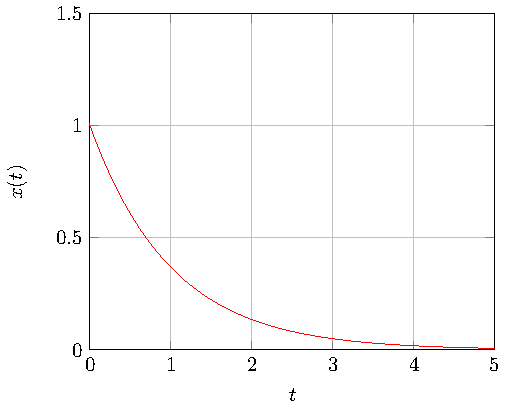
\includegraphics{ampmt_figure.pdf}
  \caption{Example of the time evolution of the model~\eqref{eq:student} with
    $x_0=1$ and $a=1$.}
  \label{fig:student}
\end{figure}

The model~\eqref{eq:student} lacks
\begin{itemize}
\item recovery of the motivation because of the progress of the research
  and tea break;
\item final stretch before the deadline.
\end{itemize}

Let us improve the model~\eqref{eq:student}.
...

\subsection{Modeling of master's thesis}
...

\section{Development of efficient algorithms}
In this section, we develop efficient algorithms for writing the master's thesis.
...

\section{Conclusion}
In this thesis, we have constructed the mathematical models of students
who write the master's thesis.
We have developed efficient algorithms for writing the master's thesis
based on the models and generated this thesis using the proposed algorithms.
The experiments have shown that the proposed algorithms generate the thesis
65536 times more efficiently than writing by oneself.

%%% Acknowledgments %%%%%%%%%%%%%%%%%%%%%%%%%%%%%%%%%%%%%%%%%%%%%%%%%%%%%%%%%%%%%
\acknowledgment
The author would like to express his sincere gratitude to Professor
Taro Joho and Assistant Professor Jiro Kogaku for their helpful advices.

%%% References %%%%%%%%%%%%%%%%%%%%%%%%%%%%%%%%%%%%%%%%%%%%%%%%%%%%%%%%%%%%%%%%%%
\addcontentsline{toc}{section}{\refname} % Add to the table of contents.
                                         % Delete if you use chapter option.
\begin{thebibliography}{10}
\bibitem{polya1945}
  G.~Polya, \textit{How to solve it: a new aspect of mathematical method},
  Princeton University Press, Princeton, 1945.
\bibitem{suuri2010}
  H.~Suri, \textit{A study on mathematical models and their validity},
  Master's thesis, Graduate School of Informatics, Kyoto University, 2010.
\end{thebibliography}
%%% If you want to use BibTeX, delete the above and insert code here.
%% \bibliographystyle{...}
%% \bibliography{...}

%%% Appendix %%%%%%%%%%%%%%%%%%%%%%%%%%%%%%%%%%%%%%%%%%%%%%%%%%%%%%%%%%%%%%%%%%%%
%%% If you don't need appendices, delete the below.
\appendix

\section{Appendix}
This is an appendix. This is a citation~\cite{polya1945}.

\begin{table}[htbp]
  \caption{This is a table.}
  \centering
  \begin{tabular}{c|cc}
      &  A  &  B \\
    \hline
    C &  70 & 80 \\
    D & 100 &  0
  \end{tabular}
\end{table}

%%% End of body %%%%%%%%%%%%%%%%%%%%%%%%%%%%%%%%%%%%%%%%%%%%%%%%%%%%%%%%%%%%%%%%%
\fi
\ifoutputcover
\cleardoublepage
%%% Covers and abstract for submission %%%%%%%%%%%%%%%%%%%%%%%%%%%%%%%%%%%%%%%%%%
\makecover                      % Cover
\makespine[\numberofspines]     % Spine
\fi
\ifoutputabstractforsubmission
\makeabstractforsubmission      % Abstract for submission
\fi
\end{document}
